\documentclass{sigchi}

% Use this section to set the ACM copyright statement (e.g. for
% preprints).  Consult the conference website for the camera-ready
% copyright statement.

% Copyright
\CopyrightYear{2017}
%\setcopyright{acmcopyright}
\setcopyright{acmlicensed}
%\setcopyright{rightsretained}
%\setcopyright{usgov}
%\setcopyright{usgovmixed}
%\setcopyright{cagov}
%\setcopyright{cagovmixed}
% DOI
%\doi{http://dx.doi.org/10.475/123_4}
% ISBN
%\isbn{123-4567-24-567/08/06}
%Conference
%\conferenceinfo{CHI'16,}{May 07--12, 2016, San Jose, CA, USA}
%Price
%\acmPrice{\$15.00}

% Use this command to override the default ACM copyright statement
% (e.g. for preprints).  Consult the conference website for the
% camera-ready copyright statement.

%% HOW TO OVERRIDE THE DEFAULT COPYRIGHT STRIP --
%% Please note you need to make sure the copy for your specific
%% license is used here!
% \toappear{
% Permission to make digital or hard copies of all or part of this work
% for personal or classroom use is granted without fee provided that
% copies are not made or distributed for profit or commercial advantage
% and that copies bear this notice and the full citation on the first
% page. Copyrights for components of this work owned by others than ACM
% must be honored. Abstracting with credit is permitted. To copy
% otherwise, or republish, to post on servers or to redistribute to
% lists, requires prior specific permission and/or a fee. Request
% permissions from \href{mailto:Permissions@acm.org}{Permissions@acm.org}. \\
% \emph{CHI '16},  May 07--12, 2016, San Jose, CA, USA \\
% ACM xxx-x-xxxx-xxxx-x/xx/xx\ldots \$15.00 \\
% DOI: \url{http://dx.doi.org/xx.xxxx/xxxxxxx.xxxxxxx}
% }

% Arabic page numbers for submission.  Remove this line to eliminate
% page numbers for the camera ready copy
% \pagenumbering{arabic}

% Load basic packages
\usepackage{balance}       % to better equalize the last page
\usepackage{graphics}      % for EPS, load graphicx instead 
\usepackage[T1]{fontenc}   % for umlauts and other diaeresis
\usepackage{txfonts}
\usepackage{mathptmx}
\usepackage[pdflang={en-US},pdftex]{hyperref}
\usepackage{color}
\usepackage{booktabs}
\usepackage{textcomp}

\usepackage[ngerman]{babel}

% Some optional stuff you might like/need.
\usepackage{microtype}        % Improved Tracking and Kerning
% \usepackage[all]{hypcap}    % Fixes bug in hyperref caption linking
\usepackage{ccicons}          % Cite your images correctly!
% \usepackage[utf8]{inputenc} % for a UTF8 editor only

% If you want to use todo notes, marginpars etc. during creation of
% your draft document, you have to enable the "chi_draft" option for
% the document class. To do this, change the very first line to:
% "\documentclass[chi_draft]{sigchi}". You can then place todo notes
% by using the "\todo{...}"  command. Make sure to disable the draft
% option again before submitting your final document.
\usepackage{todonotes}

% Paper metadata (use plain text, for PDF inclusion and later
% re-using, if desired).  Use \emtpyauthor when submitting for review
% so you remain anonymous.
\def\plaintitle{Smart Shelf: Report}
\def\plainauthor{Kevin Denk, Md. Abdul Kadir, Atika Akmal}
\def\emptyauthor{}
\def\plainkeywords{Smart Fabrication, Smart, Shelf, Drawer, HCI, Human Computer Interaction, Physical Computing}
\def\plaingeneralterms{Project Proposal}

% llt: Define a global style for URLs, rather that the default one
\makeatletter
\def\url@leostyle{%
  \@ifundefined{selectfont}{
    \def\UrlFont{\sf}
  }{
    \def\UrlFont{\small\bf\ttfamily}
  }}
\makeatother
\urlstyle{leo}

% To make various LaTeX processors do the right thing with page size.
\def\pprw{8.5in}
\def\pprh{11in}
\special{papersize=\pprw,\pprh}
\setlength{\paperwidth}{\pprw}
\setlength{\paperheight}{\pprh}
\setlength{\pdfpagewidth}{\pprw}
\setlength{\pdfpageheight}{\pprh}

% Make sure hyperref comes last of your loaded packages, to give it a
% fighting chance of not being over-written, since its job is to
% redefine many LaTeX commands.
\definecolor{linkColor}{RGB}{6,125,233}
\hypersetup{%
  pdftitle={\plaintitle},
% Use \plainauthor for final version.
%  pdfauthor={\plainauthor},
  pdfauthor={\emptyauthor},
  pdfkeywords={\plainkeywords},
  pdfdisplaydoctitle=true, % For Accessibility
  bookmarksnumbered,
  pdfstartview={FitH},
  colorlinks,
  citecolor=black,
  filecolor=black,
  linkcolor=black,
  urlcolor=linkColor,
  breaklinks=true,
  hypertexnames=false
}

% create a shortcut to typeset table headings
% \newcommand\tabhead[1]{\small\textbf{#1}}

% End of preamble. Here it comes the document.
\begin{document}

\title{\plaintitle}

\numberofauthors{3}
\author{%
	\alignauthor{Md. Abdul Kadir\\
		\affaddr{Saarland University}\\
		\affaddr{Saarbr{\"u}cken, Germany}\\
		\email{maktareq@gmail.com}}\\
  \alignauthor{Kevin Denk\\
    \affaddr{Saarland University}\\
    \affaddr{Saarbr{\"u}cken, Germany}\\
    \email{denk.kevin@web.de}}\\
  \alignauthor{Atika Akmal\\
    \affaddr{Saarland University}\\
    \affaddr{Saarbr{\"u}cken, Germany}\\
    \email{atikaakmal19@gmail.com}}\\
}

\maketitle

\begin{abstract}
  We are on the apex of interaction technology integration with every analogue system that is used in our daily life. 
  Working in big lab with lot of consumable equipments or finding a product in a supermarket is really a big deal. 
  It's really hard for a person to find an object from a gigantic shelf. 
  Also, it's hard to keep supply continuous of consumables by checking every individual slots.
  Sometime, it's impossible. 
  To ease the hard work of management and user we introduce \textit{Smart Shelf} that will bring smoothest interaction between shelf and human.
  Here, we present the overall framework, related work and the time line to implement a prototype of \textit{Smart Shelf}. 
\end{abstract}

\category{H.5.m.}{Information Interfaces and Presentation
  }{Human Computer Interaction}

\keywords{\plainkeywords}

\section{Introduction}
Today the word \textit{Smart} is almost everywhere. There are \textit{Smart Homes} and \textit{Smart Fabrication}. 
But from the last few years, HCI researchers have developed new interactive interfaces, synthesize from different perspective of humans for example Psychology, Economically and Social that can be integrated with modern technologies (Ubiquitous technology). 
People prefer to use these technologies, but sometimes face problems to obtained desired results. 
For example, most of the time people don't like to use shelves, because it is hard to find the desired item. 
By using ubiquities technology, combined with technologies of the \textit{Smart Home} and \textit{Smart Fabrication} domain an interactive shelf, called \textit{Smart Shelf}, can be developed. 
This shelf can enhance the utility of regular shelves. 
This paper describes the approach of the implementation of the \textit{Smart Shelf}. 
Different approaches of the interactive design, how the \textit{Smart Shelf} is implemented and how to interact with it is discussed. 
One focus is the interaction of users and operators with the shelf. 
In the end there is an evaluation of the design decisions regarding the project and an outlook for further work. 
The evaluation contains a short user study, too. 

\subsection{Problem}
Most people when they hear about a shelf they think about their bookshelf or some shelves in the kitchen. 
Almost everyone who have a bookshelf searched at least one time in his/her life for a book in it and wished to have a guideline how to find it the fastest way. 
Imagine big shelves with a lot of small drawers. 
Every drawer is only labelled with a small name that describes what in that drawer is. 
Searching for items in these shelves can be hard and cost a lot of time. 
An additional scenario is if you apply this concept to big warehouses with hundreds of shelves and more drawers or places where you can place items. 
Finding an item in such a warehouse can be still harder. 

Shelves used in companies or research institutes bring more problems to the surface. 
Often there are shelves used for storage of electronic components
\footnote{e.g. Resistors, Capacitor, Micro Controllers or Integrated Circuits} for example. 
The drawers contained in these shelves are often a lot and small. 
Searching for a specific item/drawer in such a shelf with for example fifty drawers can be exhausting. 
But this is not only one problem. 
Is the searched drawer found, the contained items are maybe out of stock and the user wasted his/her time for search. 
This is not only exhausting, it is also wast of time if the user could directly see if the searched item is out of stock. 
\\
\\
Not only warehouses or storage rooms with shelves have those problems with the inefficiency in finding items or the premise if one item is out of stock. 
The same problems appear in retail. 
Customers which can't find their favourite product in a shop are unsatisfied. 
Maybe they go to another shop and don't come back. 
This problem can be tackled with \textit{Smart Shelves}, too. 
The shelf itself could detect if some products in it are only available in a small amount. 
In this case the shelf could order new products or at least send an information to an operator who can order supplies. 
With this strategy there will be no more empty shelves in shops and customers can find their favourite product all the time. 
This strategy is very similar to the current trend of automation called \textit{Industrie 4.0}.
\\
\\
\textit{Smart Shelf} should be a solution for these problems. 
It could observe the amount of items in itself, help people to find products and also order supplies if the amount of items is low. 
The project described by this paper tries to give a solution for the mentioned problems. 

\section{Related Work}
There are several development work happened last few year in human computer interaction(HCI), home automation and embedded technology. A big set of these work is giving intelligence to rigid objects and allow human to communicate with them and vice-versa by applying noble HCI techniques. Moreover, post-WIMP devices also offer some features that can be integrate with the modern computer technology development(Ubiquitous computing). However, this post-WIMP GUI concept only applicable if there is a metaphor available in digital or analogue world. For example, searching the meaning of a word in digital dictionary(e.g:Smart phone dictionary). We want explain decent amount of successful research work that overlap at least in certain area with our Smart Shelf framework; However, there is no implementation or ground work fully overlap with our concept. A technical definition of our project is "Combining different interaction technique to innovate a device that follow the guideline of ubiquitous computing".The most related topic that are already known by design community are: QR code for presenting information, Automatic amount calculation, Controlling device.    
\subsection{QR code for presenting information}
Now a days application of QR code become very popular and common due to the smart phone technology. Now people don't need to type search. Pressing a key is enough to get information based on QR code. A very innovative application is using QR code in library management. In a case study ` `Application of QR Code Technology in providing Library and Information Services in Academic Libraries'' by  Sandeep
Kumar Pathak showed that important information can be presented by QR code and user can easily get all those information by scanning QR code. 
We are implying this idea in to completely different perspective. In our case every drawer will have individual QR code. Each code will represent individual information about items stored in the drawer. 
\subsection{Automatic amount calculation}
One major objective our implementation is representing empty or not empty drawer. As it's a very ground level work of many automation project, there are many project information available regarding weight measurement. However, in our project we are counting the objects based on the overall weight. We don't see this sort of work is not very common to automation community.Although, the most related work to that sub task is counting weight based on resistive sensor. An example of this work presented in $circuitdigest.com$:Arduino Weight Measurement using Load Cell and HX711 Module. Here they use Load Cell, but we will use resistive load sensor to calculate the weight signal.Also, their project does not include counting.
\subsection{Controlling Device}
The most important human to machine interaction task in this project is giving command to the system. There are several way to build up the this interaction system:one could be developing from scratch and another is building up over existing individual system. It's very common in Internet of Things (IoT) community to to use a smart phone for controlling a electronic system.For example there are lot of projects that use android devices for home automation. However, Our approach is similar but objective is completely different.
\\
\\
We see there are many existing work happened in granular level, but here we are bringing these granular ideas to build completely a new noble system.


\section{Concept}
This section describes the basic concept of the \textit{Smart Shelf}. 
The basic idea of the Smart Shelf is to enhance the interaction with shelves to work with these more effective and to improve the interaction. 
To satisfy these objectives some core features are proposed in this section. 
Figure \ref{fig:example_shelf} shows a similar shelf to the one used for the project prototype which is small but satisfies the requirements for this prototype. 
However, one important fact which should be considered is the scalability. 
The applied techniques should be feasible in a technical and economical way. 
%
\begin{figure}
	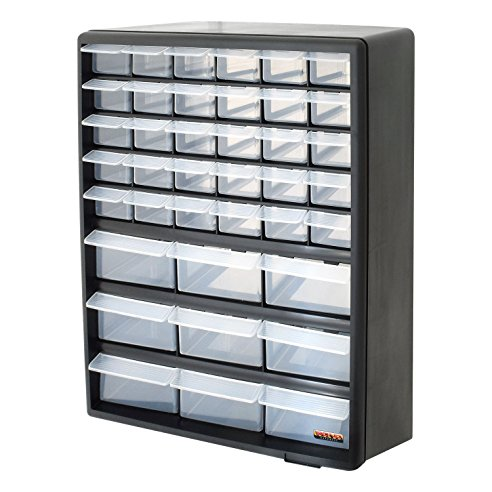
\includegraphics[width=0.9\columnwidth]{figures/example-prototype-shelf}
	\caption{Example for used Shelf as prototype}~\label{fig:example_shelf}
\end{figure}
%
\\
\\
The first problem the Smart Shelf wants to address is the fact that it is hard to find a specific item in a high amount of drawers. 
To do this we propose visual feedbacks combined with an user interface to submit search queries. 
The user interface can be used to insert a search word, for example the name of the searched item. 
This search query results in a visual feedback on the Smart Shelf, or in detail, on the specific drawer where the item is contained. 

The user interface will be provided as webapp. 
The platform independence of a webapp leads to this design decision. 
In a first iteration mobile apps are considered, but were discarded because of the platform dependency (Android, Apple iOS, Microsoft Windows, etc.). 
Additionally, more features are provided by the webapp. 
Overall, it provides all functionalities to interact with the Smart Shelf. 
The search, control the shelf or getting more data about different items. 
For getting more information about a specific item the user interface provides additionally to a datasheet-like page the capability to scan QR-Codes. 
These QR-Codes are mounted on each drawer and encode the identifier of the drawer. 
A central server, which also serves the webapp holds the state of the Smart Shelf and has a mapping of these scanned identifiers to drawers and items. 
The different items contained in the shelf, the amount of them and current searches are called here as \textit{state}. 

As mentioned before an unsatisfying fact is, if the user search for a while for a specific item and finally find it, the drawer is empty. 
To address this problem the Smart Shelf provides a \textit{predictive management system} (abbr. PMS). 
This PMS enables the system to send notifications to operators if a drawer is empty or almost empty. 
Notifications enables the operators to react early to items with low or zero amount. 
This decreases the chance of out of stock items. 
To realize such a PMS data are needed for analysis to determine different reactions. 
Every drawer will get a electronic unit to measure the weights of the items in a drawer. 
Theses measurements are send to the server, which calculates with the stored weight of the specific item, the amount of items in that drawer. 
This enables the PMS to have an overview of the state about all items contained in drawers. 
Additionally to notifications a visual feedback is given at the shelf itself. 
Empty drawers are marked with a red light to indicate this to users directly. 

As mentioned before visual feedback is a central point in the design of the Smart Shelf. 
Therefore, it is used to indicate the searched drawer to the user and if a drawer is empty. 
However, the prototype uses visual feedback additionally for a so called \textit{service mode}, which can be switched on and off.
During service mode every drawer visualizes its state with different colours. 
Blue colour, if the drawer contains more items than a specified threshold. 
Yellow colour as warning, if there are less items than the threshold and a red colour, if there are zero items left. 
For this service mode the data acquired with the weight measurement are consulted. 

\subsection{Visual Feedback Colours}
There are several ideas of giving notification for search item in drawers. For example, sound, fancy display could be used for notifying users.However, we used LED for fulfilling that purpose because LED is more catch more human attraction towards the point where led glowing compared to sound happening at a point. Moreover a display could do the the above mentioned task to notify a place, but displays are not as bright as LED  in lighting condition. Besides, implementing visual feedback system with led is cheaper than above mentioned two options So, we choose the best option, LED that fulfils our objective. Now, the problem is which colour can provide information meaningfully to user. We found red LED is the best option for giving notification about empty drawer, because culturally humans are familiar with red colour as stopping point. For example traffic light. Moreover, we have one more information to pass to user that is search item available in a specific drawer. We choice blue as a representative for that information. The reason of choosing blue is blue is visually near to the colour of green, but blue LED looks brighter than green LED. So, by breaking the cultural analogy we came up idea that a blue light could be good replacement of green light that represent availability or allowed access in real life situation. Furthermore, We allow two users using the system at the same time. We can notify empty drawers to both users by only red LEDs because the users don't have to check the drawers (No collision) if the drawer is already empty. On the other hand, if the tow users' search item is already available we must have to show them which drawer the should check out their desired items. As it mentioned blue will still used  for the for the first user, but for the second user use yellow.  The users are also notified by graphical user interface that which coloured LED give them the hint about their desired items. More description of choosing colors can be found in A Review on the Role of Color and Light in Affective Computing \cite{RefWorks:coloreffect}.

\subsection{Assumptions}
To realize this prototype some preconditions are assumed which are listed in this section. 
\\
\\
All items in the shelf are either without packaging or with packaging. 
There will be no drawer where items are mixed. 
Furthermore, at any time there is only one sort of items in one drawer. 
Every drawer contains different items. 
The weight of a specific item is stored in the server for the amount calculation. 

\section{Implementation}
This chapter shows the important details of the Smart Shelf implementation. 
The system of the Smart Shelf itself consists of three main components. 
The backend server with a MySQL database, a webapp served by the backend and Smart Shelf itself with an Arduino as main microcontroller connected to some electronic components placed in the drawers. 
Basically, the Smart Shelf is contained of several Smart Drawers. 
These components and how they communicate with each other are described in the following. 
%
\begin{figure*}
	\centering
	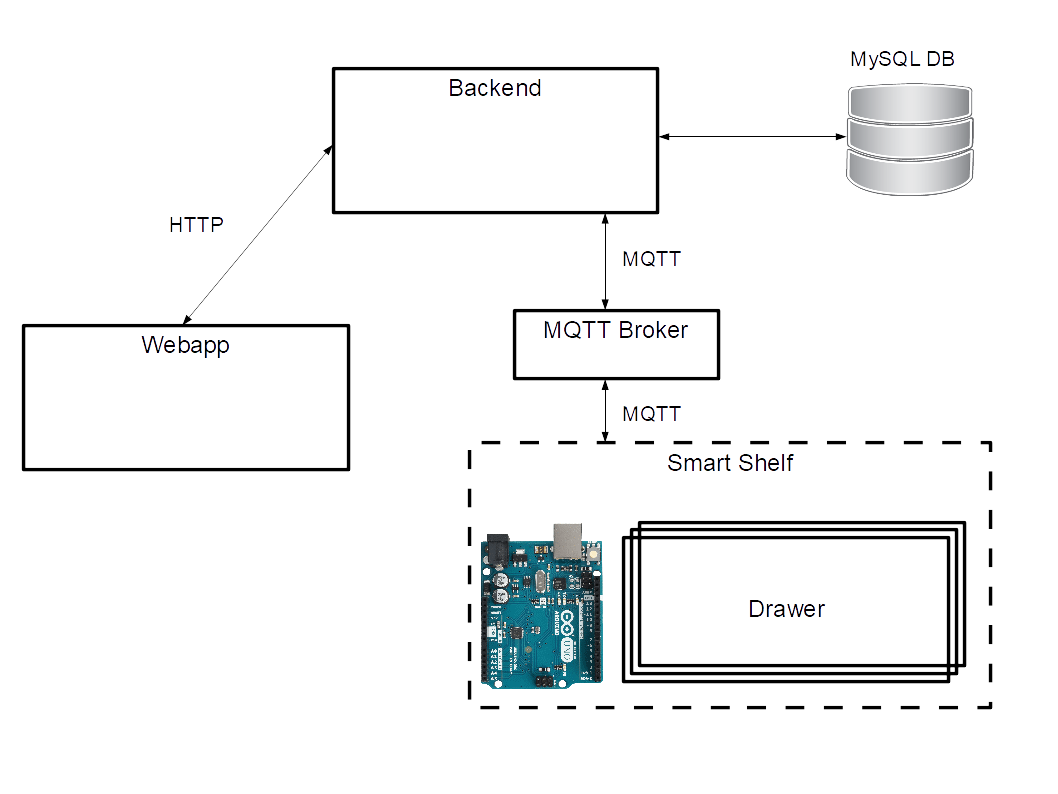
\includegraphics[width=1.3\columnwidth]{figures/infrastructure-smartshelf-white.png}
	\caption{Infrastructure of the Smart Shelf system}~\label{fig:infrastructure}
\end{figure*}
%

\subsection{Backend}
For the backend implementation the Spring framework is used. 
This enables to build a lightweight backend server that can serve web pages, a REST API and can connected to a MQTT\footnote{Abbr. Message Queuing Telemetry Transport Protocol} broker. 
The communication between backend and Arduino is explained in section \ref{sec:communciation} in detail. 
To serve the webapp the backend implements several REST Services which can be consumed via HTTP. 
Some of this services produce the different web pages for the webapp. 
Others produce just data to keep the information in the webapp up to date. 

As mentioned before the backend keeps the state of the whole system. 
For that it implements some queues for all current search queries and has a connection to a MySQL database with all the essential data needed for the Smart Shelf. 
The database contains for example all items contained in the shelf, in which drawer these items are and what boxes are there. 
Additional information like the amount of different items are stored, too. 
To enable the PMS the backend implements also some services to mark an item as out of stock and to send an email to defined operators as notification. 
These operators can subsequently order supply for the appropriate items. 
In addition to the sent notification the backend sends a command to the Arduino to switch on the red LED on that drawer. 
This signals directly to each user that this drawer is empty. 

To use more of the capabilities the visual feedback provided via the LEDs on the drawers the Smart Shelf implements a so called service mode. 
This mode can be started from the webapp. 
After started the backend checks the state of all drawers and send the appropriated commands to the Arduino to switch on the correct LED on all drawers. 
As mentioned before there is a mapping between the colours of the LED and the amount of items in a drawer. 
Blue colour signals that the amount of items in that drawer is above a defined threshold. 
Yellow colour indicates that the amount is below the threshold and red visualizes that this drawer is empty. 

\subsection{Communication}\label{sec:communciation}
For the communication between Arduino and backend the lightweight M2M\footnote{Abbr. Machine-to-Machine} communication protocol MQTT was chosen. 
MQTT works with the publish and subscribe pattern. 
There is a central broker where clients can subscribe topics. 
Additionally, clients can publish messages to different topics. 
If a client subscribed the topic under which a message is published, the client will receive it \cite{standard2014mqtt}. 
For further information about this protocol check \cite{standard2014mqtt}. 

With MQTT a bidirectional connection can be established between backend and Arduino. 
Primary, the backend send commands to the Arduino which LEDs the Arduino should switch on or off. 
But additionally, the Arduino send in a defined interval the measured weights of items contained in different drawers. 
How the weight measurement is done is explained in following chapters. 

\subsection{Smart Drawer}

\subsection{Webapp}
To control the Smart Shelf a webapp is served by the backend. 
This webapp can be opened via an URL from almost every browser which is connected to the network the backend is in. 
Implementing the user interface as webapp brings the advantage that there is no platform dependency. 
It can be used form a Android or iOS phone as well as with computer. 

Figure \ref{fig:webapp-mainpage} shows the main page of the user interface. 
%
\begin{figure*}
	\centering
	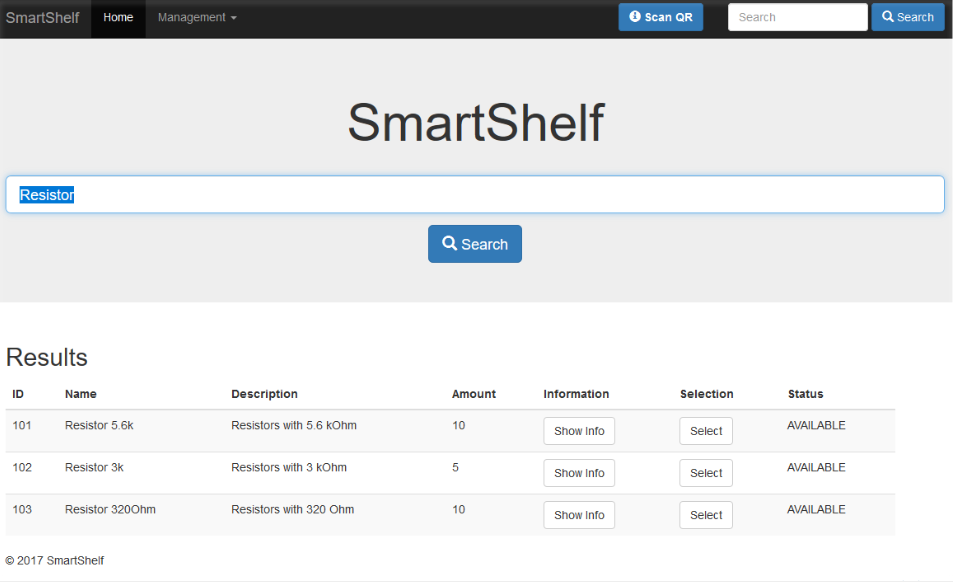
\includegraphics[width=1.3\columnwidth]{figures/ui-mainpage.png}
	\caption{Mainpage of the webapp}~\label{fig:webapp-mainpage}
\end{figure*}
%
The main function of the system is to make it easy searching for a item in the shelf. 
Therefore, a big search field can directly be seen at the main page. 
Inserting there the name of the searched item results in a list of items matching the inserted name. 
Additionally, all LEDs of the drawers which contain the displayed items in the webpage will be turned on. 
By using the "Select"-button for the item to choice all LEDs will be switched off except the selected one. 
With this functionality the user can easily find the search item without scanning the all drawers for the specific name. 

To get more information about an item one can uses the data sheet provided by the webapp. 
This can directly reached from the search result, also seen in figure \ref{fig:webapp-mainpage}, or by scanning the QR-Code mounted on the appropriate drawer. 
The QR-Code brings the advantage that if a user need more information about a specific item and is standing right in front of the shelf he/she doesn't have to search again and afterwards select the data sheet. 
The data sheet can easily get by scanning the QR-Code with the smart phone which used to operate the webapp. 
As mentioned before the QR-Code encodes the ID of the drawer. 
By scanning this ID is decoded, send to the backend which responds with the needed information about that drawer to visualize the correct data sheet. 

\section{Evaluation}
 
To evaluate interactive smart shelf, we tested it more than once time in real world scenarios. We find some strengths and weakness after the evaluation of our project. Moreover we done seven activities during evaluation that are listed in a below table.

\subsection{Strength} 
\begin{description}
  \item[$\bullet$] The design of drawers are reliable,long lasting and have Multiple User Interface.
   \item[$\bullet$] Color of LED'S follows cultural analogy, i.e. Red (no item), Blue (have an item) and Yellow (<=half amount) in each drawer.
   \item[$\bullet$] If there isn't any item or have less than half amount of an items in drawers, send notification email to administrator.
   \item[$\bullet$] Web application smoothly start service mode that depicts the current state of smart shelf.
   \item[$\bullet$] More than one user can search items simultaneously.
   \item[$\bullet$] Using QR code user can get detail information of items i.e. capacity of resistors etc.
   \end{description}
\subsection{weakness}
\begin{itemize}
  \item Keep small circuit inside each drawer is not good idea.It became messy with items even LED'S inside drawer is not clearly visible for visualization.
  \item Most important keep a plastic plate on the top of load sensor to fix load sensor inside drawer does not give proper measurement.
  \item  Power supply is also an issue, when multiple drawers connect with micro controller.
  \item Place a QR code outside of each small drawer is also a challenge.
\end{itemize}
\subsection{Best Scenarios} 
  The project works best when search any item in drawer and scan QR code to get further detail through web app. Although proper communication is established between web app and micro controller via MQTT protocol. 
\subsection{Failed Scenarios}
 Sometimes when service mode start/stop, LED'S are not properly ON/OFF because of inefficient power supply. Power supply for Arduino is crucial as it stop works at any random point of time in between of service mode which is not good. Further More load sensor does not show accurate weight of items owing to resistance in between plastic plate and drawer.
A broken of MQTT connection immediately would lead to loss of communication between Micro controller and Web app.
\subsection{User Testing} 
We tried web app Smart Shelf with different users and observe while they were doing these activities. These activities are listed in a given table below.

%\graphicspath{ {figures/table} } 

We tested all these activities with different 4 participants and get feedback about this web app. The participants were from different age groups range from 22 to 30 years old people some was employee and some were students. For each participant performed each activity 10 times as mention in table. Then we evaluated the number of successful observations, false results and no response. We calculated the percentage of successful observations for each activity and each participant perform these activities and reasons of fault results.

For activity 1 and 5, we found our system is working properly almost 99% cases was matched with accepted results according to our observation.
While for activity 2, the system was relatively less accurate as compared to the first activity. more than once time the system does not show perfect. In 81 percent cases the system measured the weight of items correctly but 19 percent the system failed to measure quantity of items. because to calculate quantity was depend on accurate weight measurement but sometimes load sensor interpret wrong weight. That's why with 3rd participant the success rate was 81 percent as compared to the 2nd one. 
Meanwhile activity 6 had high percentage of correct cases with 99 percent among the other all activities.
As we went further and test activity 4 and 5, achieved success ratio over 96 percent, 4 percent cases was failed because of incorrect operations performed by novel users.
In Contrast the last activity, 55 percent cases was failed because of the system was behave unintentionally and inefficient power supply to micro controller was also a critical issue. So the result was not fine among all of above mention activities as 72 percent cases were failed because of inefficient power supply. Participants give bad feedback when they stopped service mode the LED'S was still blinked and system became unresponsive. 
At the end we conclude overall success rate of our smart shelf web app in the light of these 7 activities was 90 percent was perfect as shown in fig (a). As this figure represent the overall evaluation report in form of chart. But 10 percent was unsatisfied owing to some reasons that is mention above.



\section{Future Work}\label{sec:future-work}
Currently, every drawers are connected with the main controller via wires. However, this wires reduce the user friendliness, if an user pull out the drawer completely. For the purpose of fast and cost effective prototype implementation we restrict ourself to implement such a sophistical system. The idea of making each drawer independent of wire is placing connection pins bottom of the drawers and also the out going wire to the controller 
should be placed with small plate in the main structure of the shelf, so that the when the drawer is closed each of the drawer get a connection between the pins and plate and make bridge between the drawers and controller.
There figure \ref{fig:connector} shows the idea of implementing such a drawer with a very minimalistic complexity.
%
\begin{figure}
	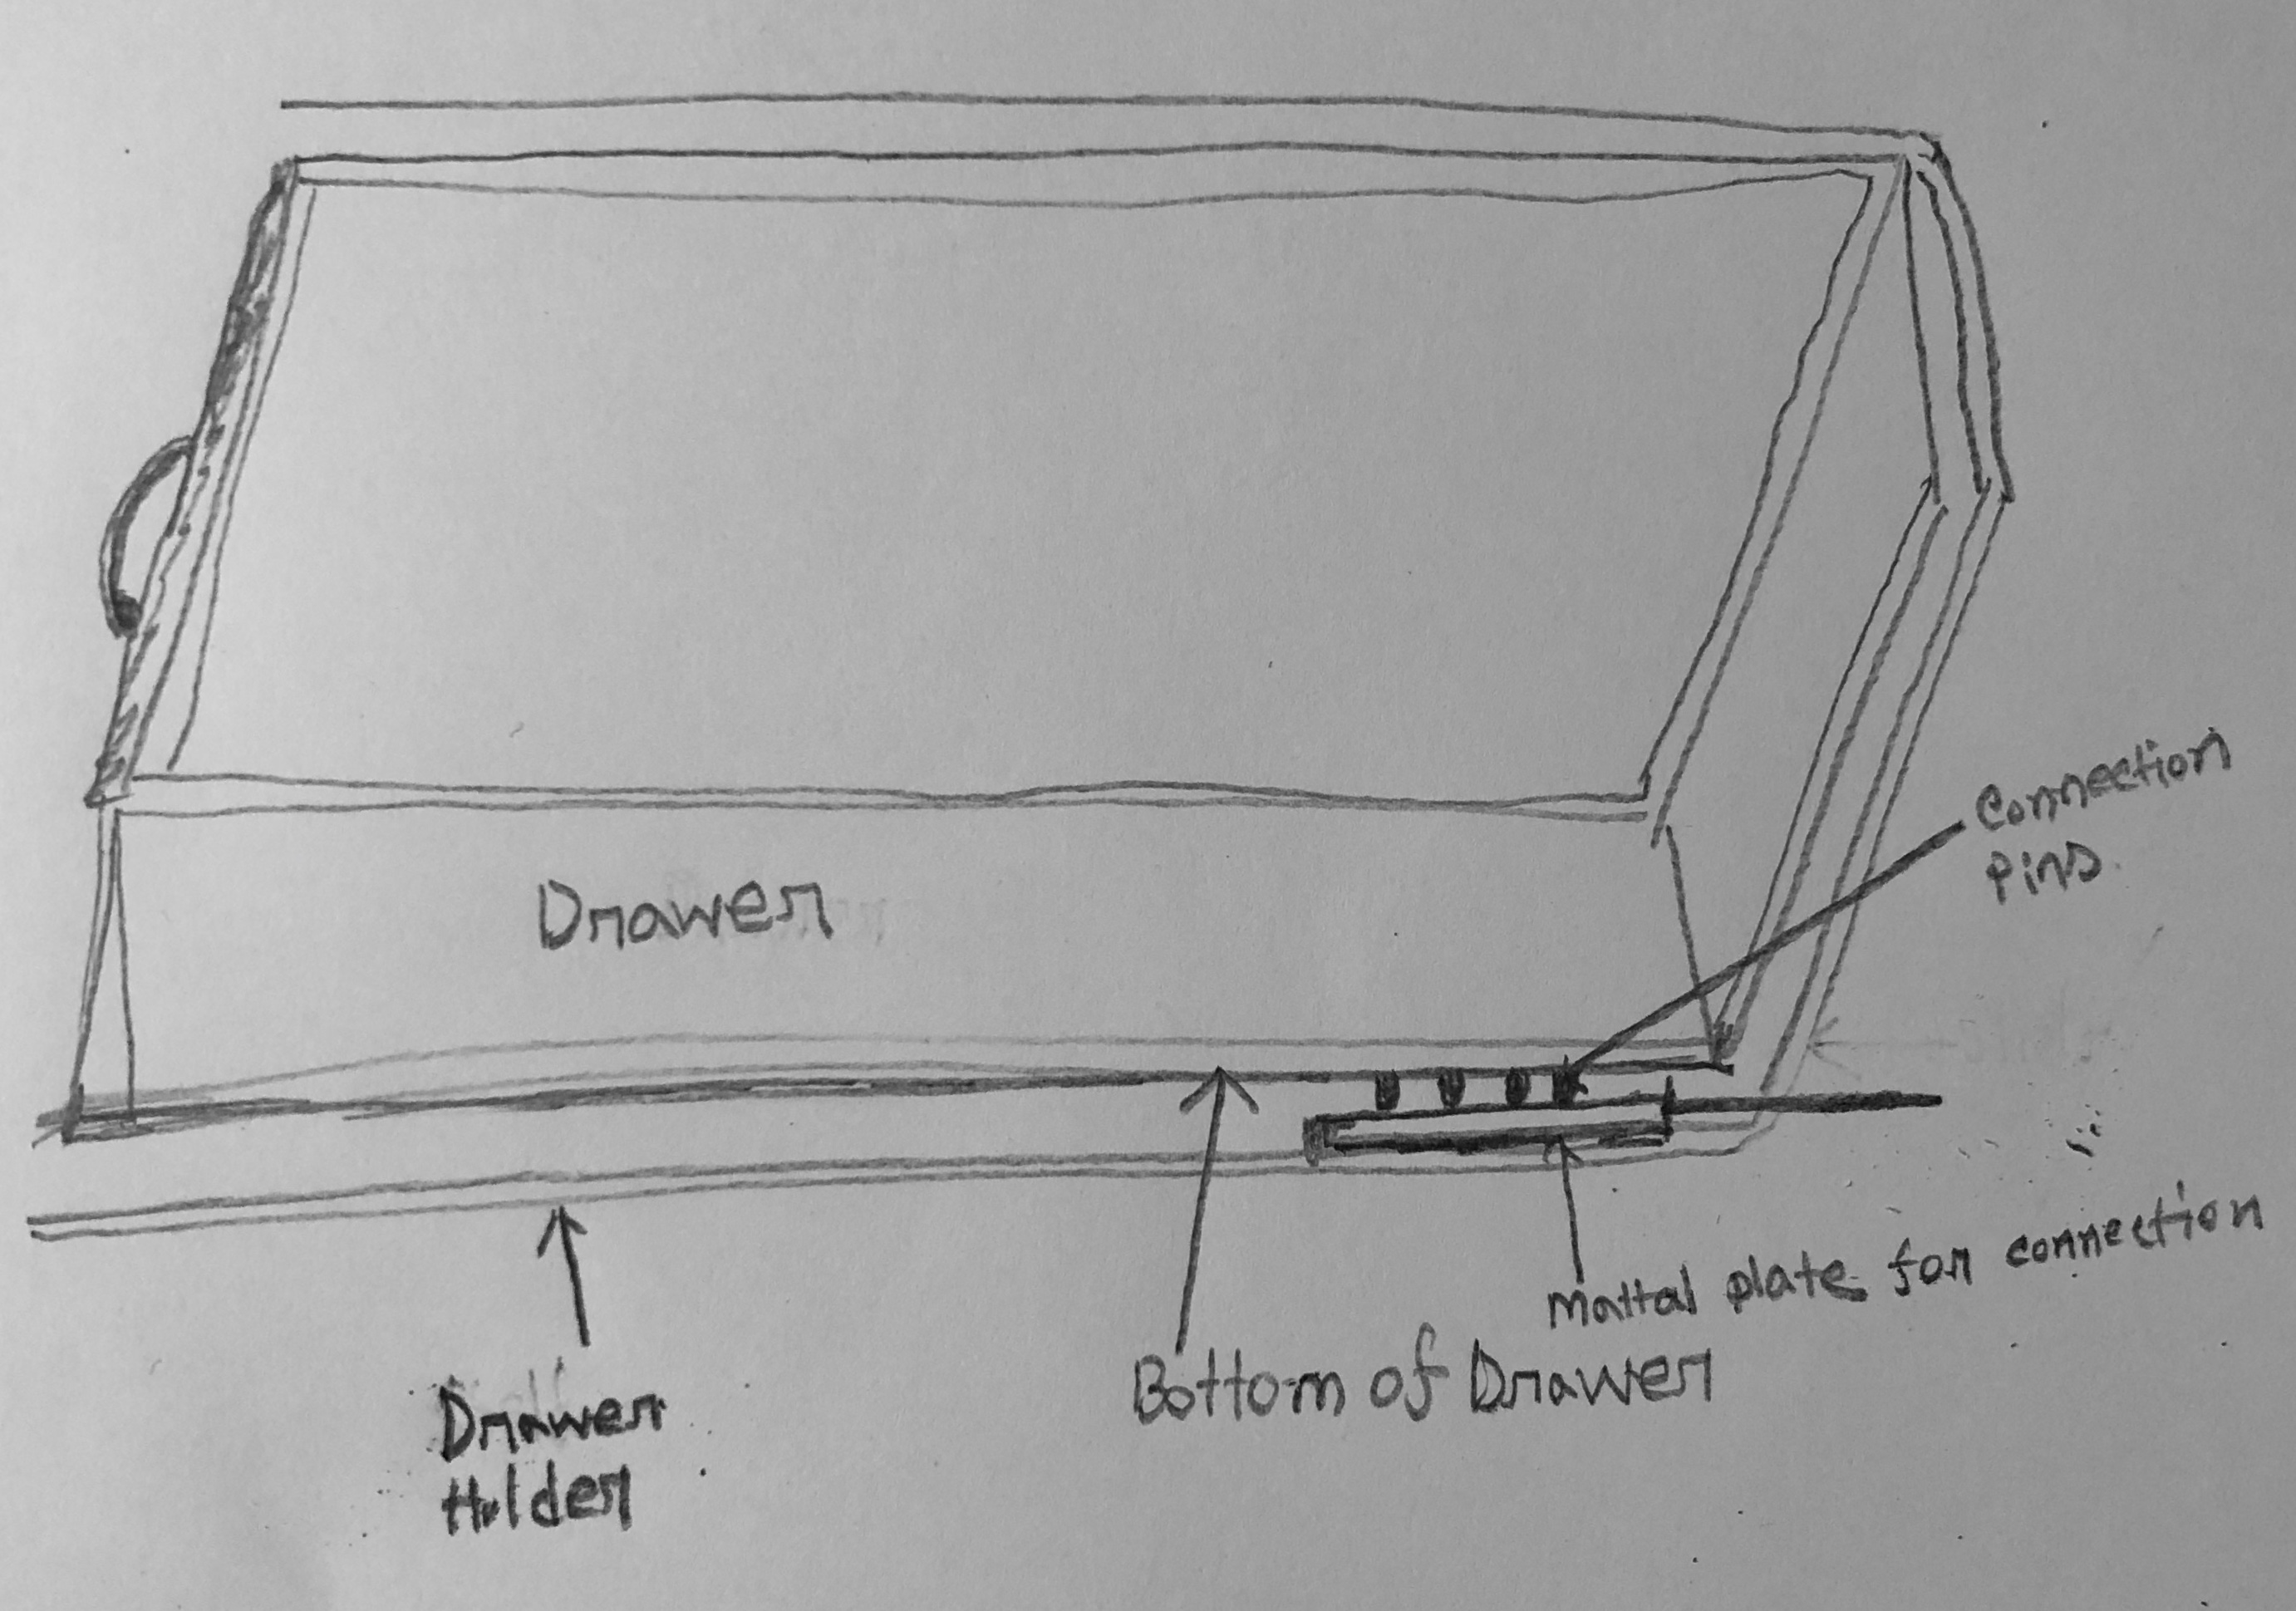
\includegraphics[width=1\columnwidth]{figures/connector}
	\caption{Sketch of connector for removing dependency on connecting wires}~\label{fig:connector}
\end{figure}
%


\section{Conclusion}
We have deployed the content of physical computing in the form of interactive smart shelf where user interact via web app and get visual feedback according to operation. Our main goal to design interactive smart shelf to reduce conscious thought while search an item as well as provide  reliable and efficient way of searching , save time and provide multiple user interface. By using Ubiquitous and other technologies, interactive smart shelf enhance the usability of shelves.


% Balancing columns in a ref list is a bit of a pain because you
% either use a hack like flushend or balance, or manually insert
% a column break.  http://www.tex.ac.uk/cgi-bin/texfaq2html?label=balance
% multicols doesn't work because we're already in two-column mode,
% and flushend isn't awesome, so I choose balance.  See this
% for more info: http://cs.brown.edu/system/software/latex/doc/balance.pdf
%
% Note that in a perfect world balance wants to be in the first
% column of the last page.
%
% If balance doesn't work for you, you can remove that and
% hard-code a column break into the bbl file right before you
% submit:
%
% http://stackoverflow.com/questions/2149854/how-to-manually-equalize-columns-
% in-an-ieee-paper-if-using-bibtex
%
% Or, just remove \balance and give up on balancing the last page.
%
\balance{}

% BALANCE COLUMNS
\balance{}

% REFERENCES FORMAT
% References must be the same font size as other body text.
\bibliographystyle{SIGCHI-Reference-Format}
\bibliography{./bib/bib}



\end{document}

%%% Local Variables:
%%% mode: latex
%%% TeX-master: t
%%% End:
